\section{SEER Data Source, Cohort Construction and Preprocessing}
\label{sec:data}

\subsection{Registry extract and relationship to the reference cohort}
\label{sec:data:source}

The source was a SEER*Stat Case Listing export from \emph{Incidence---SEER
Research Data, 17 Registries, Nov 2023 Sub (2000--2021)}, released in April
2024. The selected database is documented in the saved SEER*Stat session
screenshots and in the NCI submission documentation \citep{SEERNov2023}.
The export used diagnosis years 2010--2016. These selection years must be
distinguished from the full calendar-year coverage of the database.

The reference study used the November 2019 submission with 18 registries
and the same diagnosis-year interval \citep{Li2023}.
Consequently, the present extract is a reconstruction of the reference
eligibility framework using a different registry release, not a recovery of
the original patient-level dataset. Table~\ref{tab:data:source_comparison}
summarises the distinction. Differences in registry composition, record
updates, follow-up and implementation of exclusions may affect the resulting
cohort; their separate contributions have not been quantified here.

\begin{table}[htbp]
\centering\small
\caption{Reference-study and project data sources. Reference counts are
reported by \citet{Li2023}; project counts are from the November 2023 SEER
extract after applying the selection and preprocessing steps adapted from the
reference-study methodology.}
\label{tab:data:source_comparison}
\begin{tabularx}{\linewidth}{@{}lYY@{}}
\toprule
 & Reference study & This project \\
\midrule
SEER submission & November 2019 & November 2023 \\
Registry set & 18 registries & 17 registries \\
Database years & 2000--2017 & 2000--2021 \\
Selected diagnoses & 2010--2016 & 2010--2016 \\
Analytic cohort & 1,998 & 2,672 \\
Liver metastasis at diagnosis & 343 (17.2\%) & 462 (17.3\%) \\
External hospital data & Included in the reference study & UK--Erlangen cohort (30 patients) \\
\bottomrule
\end{tabularx}
\end{table}

The similar metastasis proportions are descriptive, not a validation criterion:
the pipeline was not adjusted to force agreement with the paper's sample size
or prevalence. The larger retained sample also cannot, on its own, establish
broader population coverage or improved representativeness.

\subsection{SEER*Stat Case Listing session and raw export}
\label{sec:data:seerstat}

The registry records were extracted with SEER*Stat software
(\url{https://seer.cancer.gov/seerstat/}), version 9.0.43.0, using a Case
Listing session. Figures~\ref{fig:data:seerstat-database} and
\ref{fig:data:seerstat-configuration} show the selected November 2023 database,
the eligibility filters and the 30 fields included in the raw export. Together,
these settings explain how the source dataset was obtained before Python
preprocessing began. The database-selection screen also shows an optional link
to county-level attributes, but none of those attributes was included among the
exported fields or used in the analyses.

\begin{figure}[p]
\centering
\begin{subfigure}[t]{\linewidth}
  \centering
  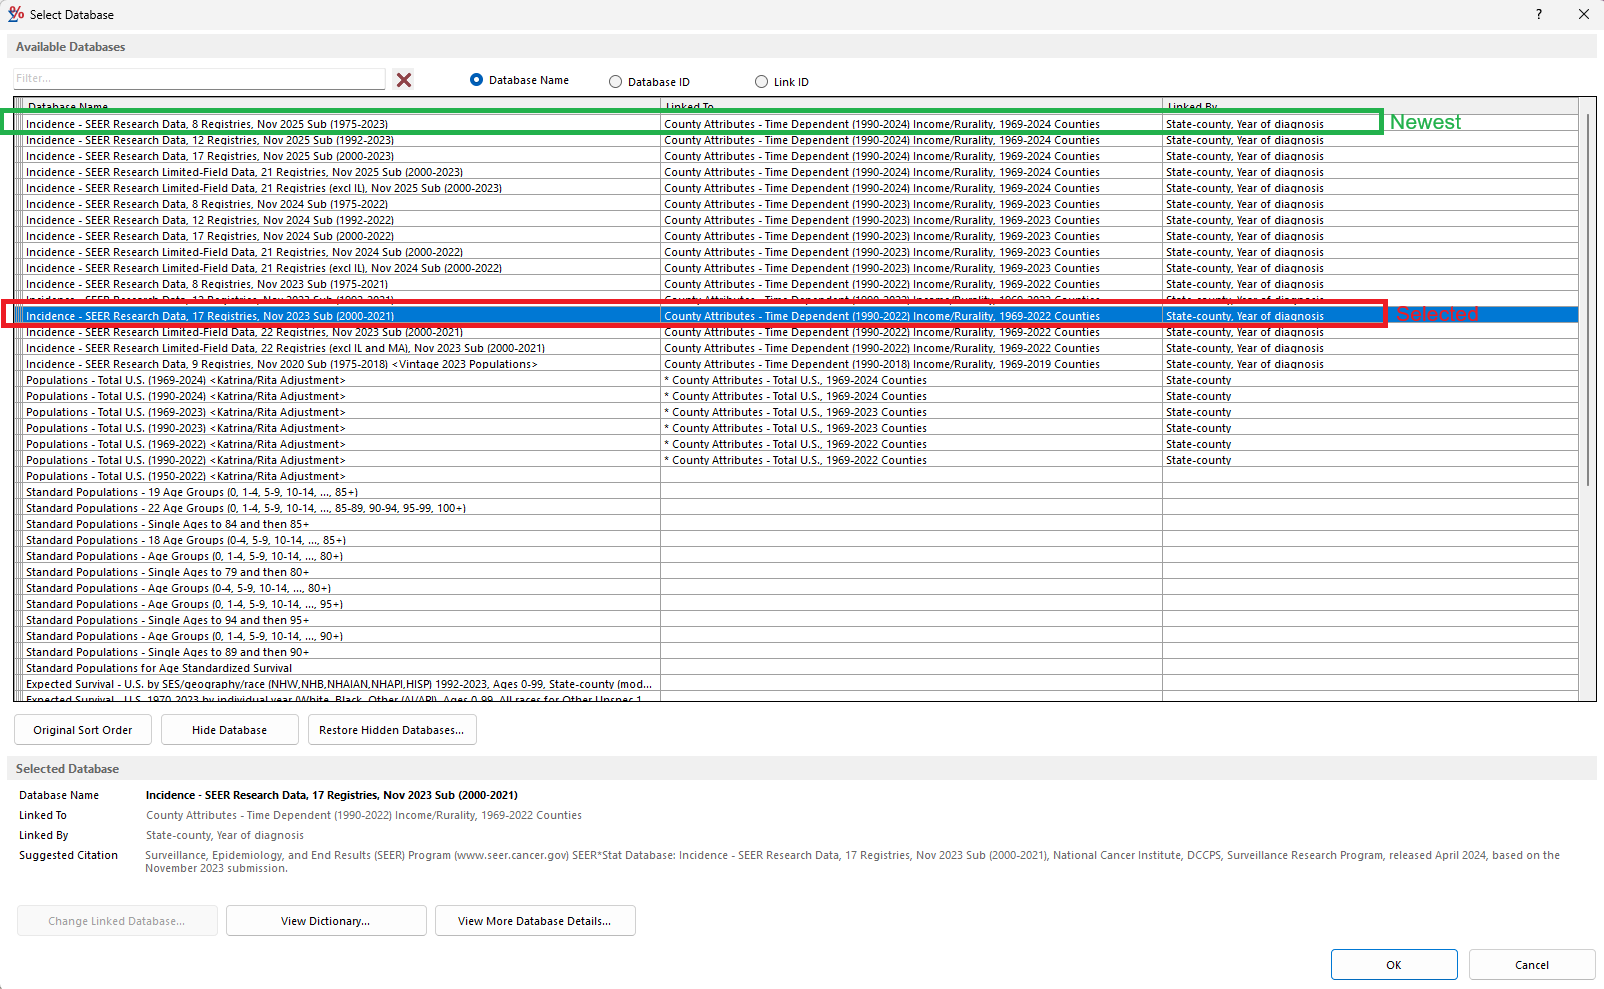
\includegraphics[width=0.98\linewidth]{data_processing/seerstat_database_selection.png}
  \caption{Database-selection dialog. The blue row and red annotation identify
  the November 2023 SEER Research Data, 17 Registries submission used in this
  project. The green annotation identifies the newest release visible when the
  capture was made, not the database used for the analysis.}
  \label{fig:data:seerstat-database-select}
\end{subfigure}

\vspace{0.8em}

\begin{subfigure}[t]{\linewidth}
  \centering
  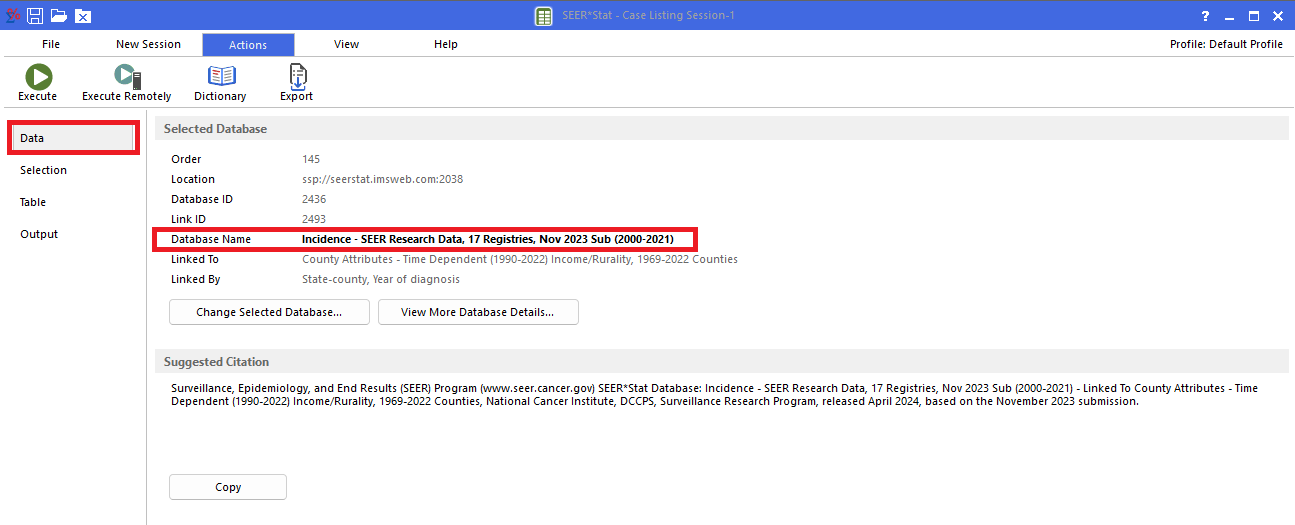
\includegraphics[width=0.92\linewidth]{data_processing/seerstat_data_tab.png}
  \caption{Case Listing Data tab confirming the November 2023 database selected
  for the export.}
  \label{fig:data:seerstat-data-tab}
\end{subfigure}
\caption{SEER*Stat database selection for this project. The November 2023
submission was used for the present analysis; the reference study used the
November 2019 submission.}
\label{fig:data:seerstat-database}
\end{figure}

\begin{figure}[p]
\centering
\begin{subfigure}[t]{\linewidth}
  \centering
  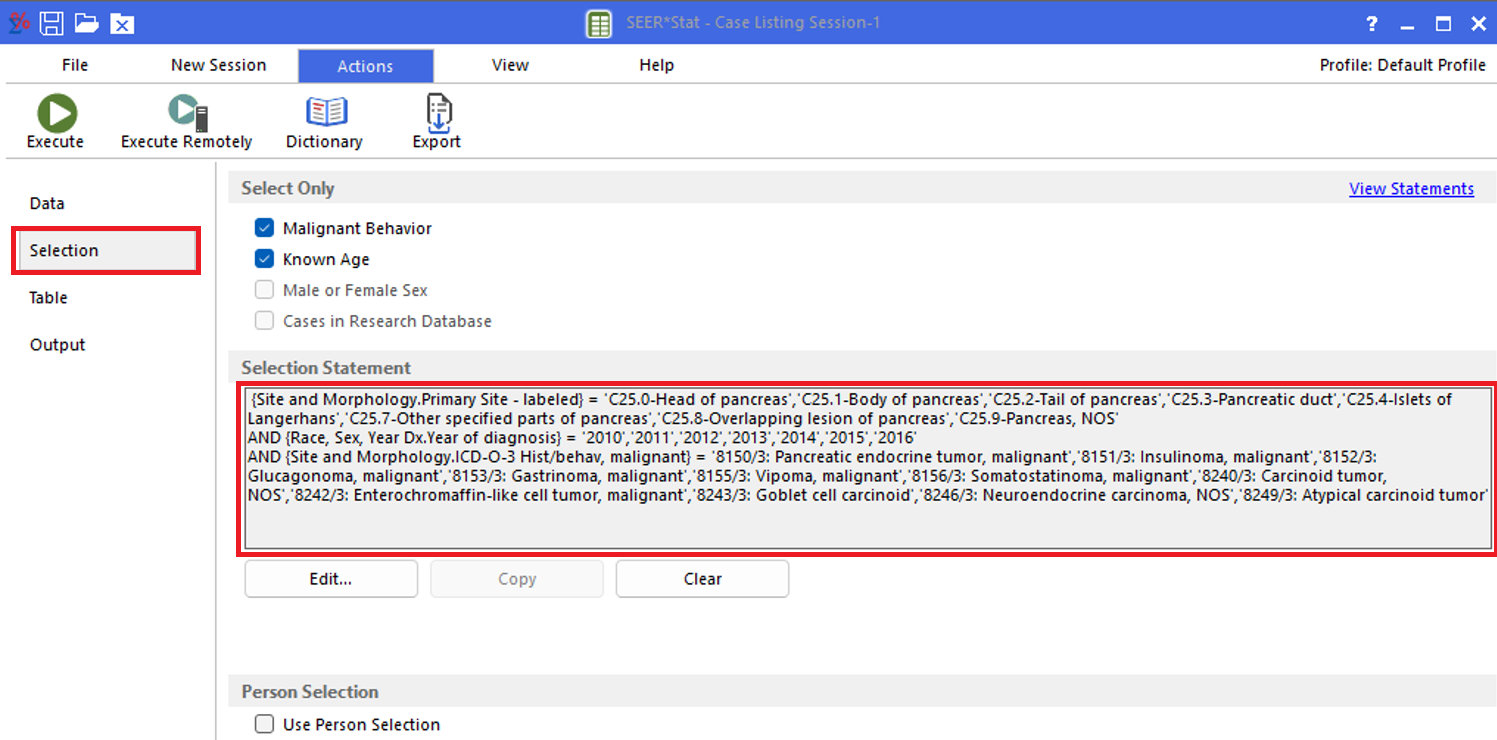
\includegraphics[width=0.98\linewidth]{data_processing/seerstat_selection_criteria.png}
  \caption{Selection tab showing malignant behaviour, known age, pancreatic
  primary-site codes, the 2010--2016 diagnosis interval and the accepted
  ICD-O-3 histology/behaviour codes.}
  \label{fig:data:seerstat-selection}
\end{subfigure}

\vspace{0.8em}

\begin{subfigure}[t]{\linewidth}
  \centering
  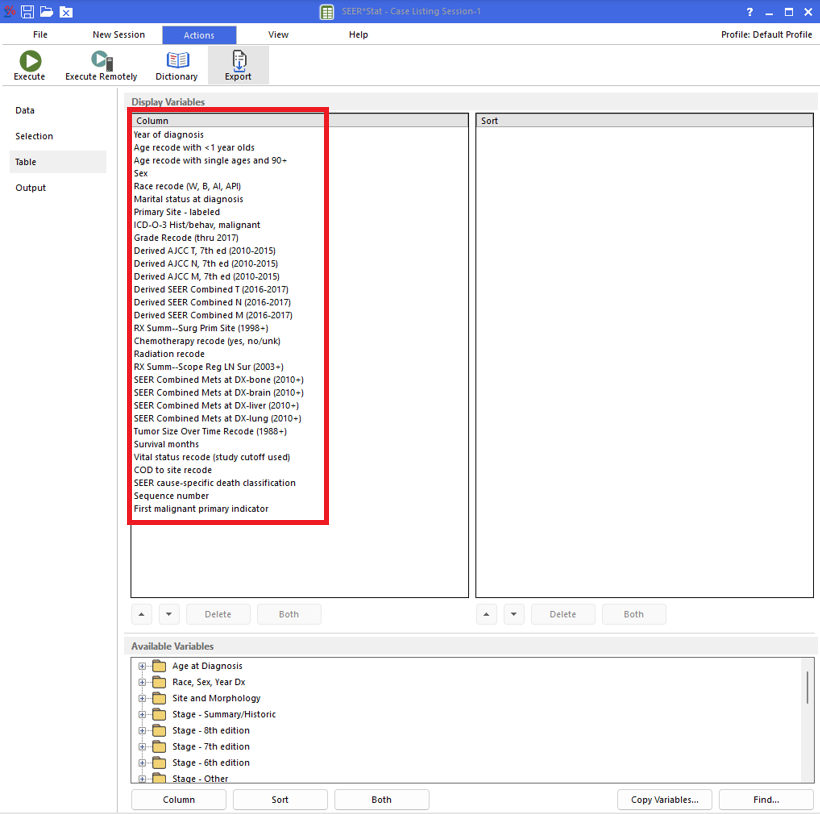
\includegraphics[width=0.64\linewidth]{data_processing/seerstat_export_variables.png}
  \caption{Table tab listing the 30 fields selected for the Case Listing
  export.}
  \label{fig:data:seerstat-table-tab}
\end{subfigure}
\caption{SEER*Stat Case Listing filters and exported fields used to create the
raw dataset before Python preprocessing.}
\label{fig:data:seerstat-configuration}
\end{figure}
\FloatBarrier

Executing the session produced \texttt{SEER\_Dataset.csv}, a UTF-8 CSV with a
byte-order mark. It contains 5,761 records and 30 fields spanning diagnosis
year, demographics, primary site, histology, differentiation, TNM sources,
treatment recodes, organ-specific metastases, tumour size, survival and
eligibility indicators. The preprocessing loader explicitly uses
\texttt{utf-8-sig} and disables pandas' default missing-value vocabulary so
that the literal value ``None'' in the lymph-node-surgery field remains a
valid source category rather than being converted to a missing value.

\subsection{Extraction criteria and record-level eligibility}
\label{sec:data:eligibility}

The saved SEER*Stat selection restricts the extract to malignant behaviour,
known age, the specified pancreatic sites and histology codes, and the
2010--2016 diagnosis interval. Accepted topography codes are C25.0, C25.1,
C25.2, C25.3, C25.4, C25.7, C25.8 and C25.9. The histology/behaviour
selection comprises 8150/3, 8151/3, 8152/3, 8153/3, 8155/3, 8156/3,
8240/3, 8242/3, 8243/3, 8246/3 and 8249/3. These are the implemented
registry categories; the \pNET{} designation in this report should not be
read as a new pathological reclassification of individual records.

Python preprocessing rechecks the year, site and histology criteria and applies
the \texttt{First malignant primary indicator = Yes} rule. This is the
configured rule, rather than an assumption that only people with a single
lifetime primary tumour are eligible. Records with an excluded cause-of-death
classification, invalid follow-up or unknown required analytic fields are
then removed in the order shown below. There is no adult-only age filter;
the retained recorded ages range from 4 to 90 years, with the upper value
including the source category of 90 years or older.

\subsection{Sequential attrition and resulting cohorts}
\label{sec:data:attrition}

Table~\ref{tab:data:attrition} shows how the number of eligible records changes
after each selection and preprocessing step.
The year, pancreatic-site and histology checks remove no further records
because the export already satisfies those criteria. The largest subsequent
exclusion is the removal of 1,903 records with at least one unknown required
analytic field: 41.6\% of the 4,575 records reaching that step. Overall,
2,672 of the 5,761 exported records are retained (46.4\%).

\begin{table}[htbp]
\centering\small
\caption{Sequential preprocessing exclusions. Each row shows the number of
records removed at that step and the number remaining.}
\label{tab:data:attrition}
\begin{tabularx}{\linewidth}{@{}rYrr@{}}
\toprule
Step & Criterion & Removed & Remaining \\
\midrule
0 & Raw SEER export & --- & 5,761 \\
1 & Diagnosis year 2010--2016 & 0 & 5,761 \\
2 & First malignant primary indicator & 1,150 & 4,611 \\
3 & Accepted pancreatic primary site & 0 & 4,611 \\
4 & Accepted histology/behaviour code & 0 & 4,611 \\
5 & Exclude unclear cause-of-death classification & 26 & 4,585 \\
6 & Exclude invalid or incomplete follow-up & 10 & 4,575 \\
7 & Exclude unknown required analytic fields & 1,903 & 2,672 \\
\bottomrule
\end{tabularx}
\end{table}

The complete-case criterion covers 20 fields: age, sex, race, marital status,
histology code, grade, primary site, T stage, N stage, primary-site surgery,
lymph-node surgery, chemotherapy, radiotherapy, four organ-metastasis indicators,
tumour size, survival months and vital status. M stage is retained for reference
in the full dataset but is not a required field in this run. The exclusion
rule removes a record if at least one of these required fields is unknown, and
one record may contain unknown values in several fields.

Figure~\ref{fig:data:flow} distinguishes the final analytic cohort from its
liver-metastasis subset. The diagnostic and prognostic datasets are not
independent samples: the latter is nested within the former.

\begin{figure}[htbp]
\centering
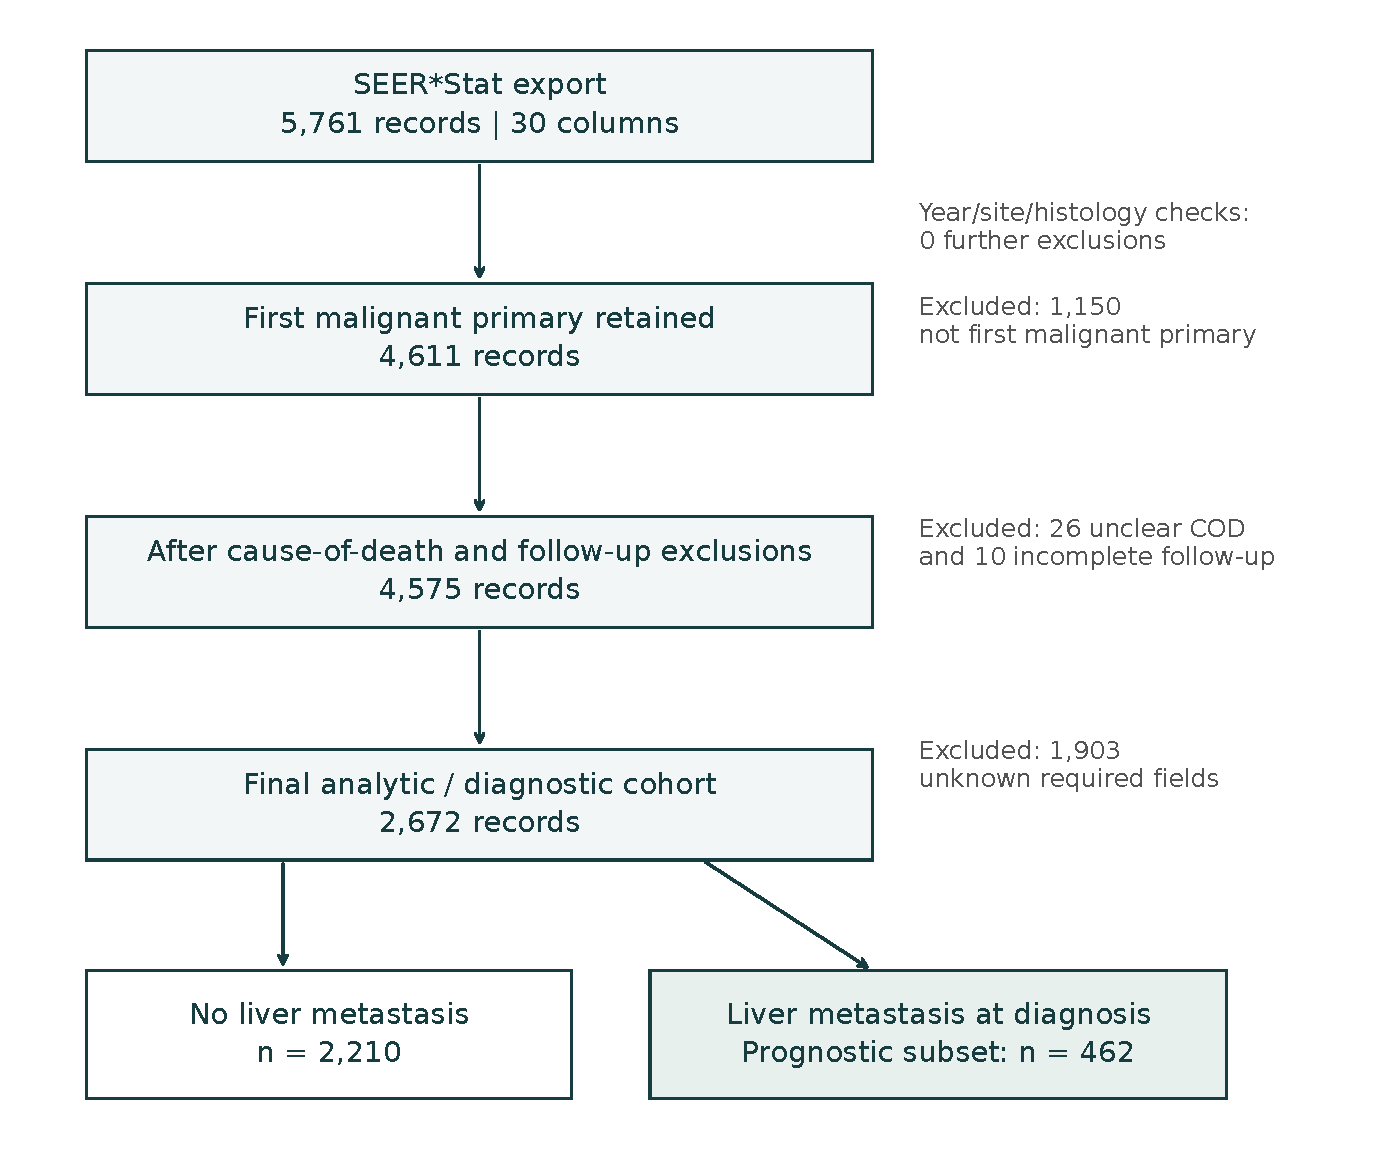
\includegraphics[width=\linewidth]{data_processing/cohort_flow.pdf}
\caption{Cohort construction from the exported records. COD: cause of death.
Both liver-metastasis groups contribute to the diagnostic task; only the 462
liver-positive records enter the prognostic task. Counts refer to this extract,
not the reference paper.}
\label{fig:data:flow}
\end{figure}

\subsection{Task definitions and analytic outputs}
\label{sec:data:tasks}

Three complementary files are produced: a full analytic table with
2,672 rows and 38 columns, a diagnostic table with 2,672 rows and 21 columns,
and a prognostic table with 462 rows and 23 columns. Column totals include
identifiers, targets and alternative encodings; they are not the number of
independent predictors supplied to every model.

For diagnosis, the binary target is liver metastasis at diagnosis
(\texttt{mets\_liver}): 462 positive and 2,210 negative records.
General M stage and its binary encoding are excluded from the diagnostic
file because they encode related metastatic status. Survival outcomes are
also absent from this task-level file. Removing these fields prevents the
diagnostic models from using information that directly reveals or closely
reflects the target. Treatment variables remain available, but the registry
does not establish whether each treatment was already known at the intended
prediction time.

For prognosis, eligibility requires \texttt{mets\_liver = 1}. Overall
survival is represented by the recorded months from diagnosis and an event
indicator equal to 1 for death from any cause and 0 for an alive/right-censored
record. The prognostic dataset contains 311 patients who died and 151 whose last
recorded status was alive, so their survival times are right-censored. Recorded
follow-up ranges from 0 to 143 months, including 12 patients with zero recorded
months. These values are kept as recorded. If a survival method requires a
strictly positive time, the necessary adjustment is made and reported within
that model's analysis. The observed range alone does not describe the typical
follow-up time or median survival of the cohort.

\begin{table}[htbp]
\centering\small
\caption{Selected characteristics of the diagnostic and prognostic datasets
obtained after cohort selection and preprocessing. Percentages use the
column-specific sample size. Q1--Q3 denotes the first and third age quartiles;
the prognostic cohort is a subset of the diagnostic cohort.}
\label{tab:data:cohort_summary}
\begin{tabularx}{\linewidth}{@{}Y>{\RaggedRight\arraybackslash}p{4.2cm}>{\RaggedRight\arraybackslash}p{3.2cm}@{}}
\toprule
Characteristic & Diagnostic & Prognostic \\
\midrule
% The expandable input primitive keeps booktabs rules aligned after imported rows.
\csname @@input\endcsname{tables/data_processing/cohort_summary_rows.tex}
\bottomrule
\end{tabularx}
\end{table}

\subsection{Clinical recoding and retained ambiguities}
\label{sec:data:recoding}

Table~\ref{tab:data:recoding} summarises how the original SEER fields were
converted into consistent variables for analysis. These rules include category
grouping, binary coding, selection between available staging fields and survival
coding, and they were applied in the same way to every eligible record. Steps
that depend on a fitted model, such as pooling rare categories, scaling or
feature selection, were performed later using only the relevant training data.

\begingroup
\small
\setlength{\tabcolsep}{5pt}
\begin{longtable}{@{}>{\RaggedRight\arraybackslash}p{3.1cm}>{\RaggedRight\arraybackslash}p{6.3cm}>{\RaggedRight\arraybackslash}p{5.1cm}@{}}
\caption{Principal clinical recoding rules used to prepare the analysis
datasets.}
\label{tab:data:recoding}\\
\toprule
Domain & Implemented representation & Interpretation or limitation \\
\midrule
\endfirsthead
\multicolumn{3}{l}{\textit{Table \thetable\ continued}}\\
\toprule
Domain & Implemented representation & Interpretation or limitation \\
\midrule
\endhead
\midrule
\multicolumn{3}{r}{\textit{Continued on next page}}\\
\endfoot
\bottomrule
\endlastfoot
Demographics & Single-year age; male indicator; four recorded race categories;
married versus other known marital categories. & Age 90+ is stored as 90.
Unknown race or marital status is excluded, not imputed. \\[0.6em]
Histology & Diagnostic labels retain the accepted histology categories.
Prognosis groups codes 8240/3 and 8249/3 as ``Carcinoid tumor'', with other
accepted codes grouped as ``Others''. & The binary prognostic grouping is an
analysis convention, not equivalence of the underlying histologies. \\[0.6em]
Differentiation & Legacy grade recode mapped to integers 1--4; unknown grade
excluded. & These are the registry differentiation categories, not a newly
derived Ki-67/mitotic-count classification. \\[0.6em]
Anatomic site & Pancreatic head, body, tail and other accepted sites. &
The ``Others'' category combines several source sites. \\[0.6em]
T and N stage & Prefer AJCC 7th-edition values for 2010--2015 and SEER Combined
values for 2016; use a valid alternative source as fallback. Clinical/pathological
prefixes are collapsed to T0--T4 and N0/N1. & Combining the available staging
fields provides consistent model inputs across diagnosis years, but differences
between clinical and pathological assessment are no longer retained. N1 is
additionally encoded as \texttt{n\_stage\_positive}. \\[0.6em]
Primary surgery & Code 00 is 0; code 99 is missing; other parsed nonzero codes
are 1. & Procedure detail and timing are lost in the binary representation. \\[0.6em]
Lymph-node surgery & ``None'' is 0; biopsy, removal and sentinel-node categories
are 1. ``Unknown or not applicable'' is missing. & Not inferred from the absence
of primary-site surgery; a positive value is not a lymph-node tumour finding. \\[0.6em]
Chemotherapy & ``Yes'' is 1; ``No/Unknown'' is 0. & Zero does not establish
that chemotherapy was not received. \\[0.6em]
Radiotherapy & Active radiation categories are 1; ``None/Unknown'' and
``Refused'' are 0. ``Recommended, unknown if administered'' is missing. &
The zero category combines different treatment-information states. \\[0.6em]
Tumour size & Store numerical millimetres and groups
$0\leq s\leq26$, $26<s\leq36$, and $s>36$. Unknown/unreasonable labels are
missing. & The stored label ``26--36 mm'' excludes exactly 26 mm.
Code 000 is retained as 0, not an unknown value. \\[0.6em]
Organ metastases & Bone, brain, liver and lung fields: Yes = 1, No = 0;
unknown values excluded. & Liver status is the diagnostic outcome and
prognostic eligibility criterion, not a prognostic predictor. \\[0.6em]
Survival & Numerical months; Dead = 1 and Alive = 0. & All-cause mortality,
not cancer-specific survival; zero-month records remain in the input. \\
\end{longtable}
\endgroup

Treatment information deserves particular caution. NCI documentation states
that these chemotherapy and radiotherapy variables concern first-course
treatment and that non-recording cannot reliably distinguish no treatment
from unknown treatment \citep{SEERTreatment2023}. The report therefore retains
the mixed meanings of the zero codes rather than describing them simply as
untreated patients. The exported fields also do not establish that treatment
was known before the intended diagnostic or prognostic prediction time.

\subsection{Data checks and implications for downstream evaluation}
\label{sec:data:checks}

Before modelling, the processed data were checked to confirm that the exclusion
steps lead to the final cohort of 2,672 records, that the diagnostic dataset
contains all retained patients and that the prognostic dataset contains exactly
the 462 patients with liver metastasis at diagnosis. The checks also confirmed
that analysis identifiers are unique and that all required fields are complete
under the implemented coding. Table~\ref{tab:data:cohort_summary} describes the
main characteristics of these two datasets.

Each retained record receives a new sequential analysis identifier after
filtering. This identifier is used only to keep the same record aligned across
datasets and model outputs. It is not the original SEER patient identifier and
cannot be used to link a patient across different SEER releases.

Four consequences constrain all later experiments. First,
complete-case selection is substantial and need not be representative of the
excluded records. Because both tasks descend from the same filtered cohort,
the diagnostic dataset also inherits follow-up and cause-of-death exclusions,
although those fields are not diagnostic predictors. Excluding an unclear
cause of death follows the reproduction workflow; it is not intrinsically
necessary to define all-cause mortality.

Second, no blank values in a task-level file does not imply complete clinical
information. Treatment ambiguity persists within the stored codes, while
stage-source harmonisation, coarse histology grouping and top-coded age reduce
detail. There is no basis for treating the retained records as missingness-free
measurements of every clinical construct.

Third, sparse strata are present even before modelling: the prognostic cohort
contains only three records with brain metastasis and 33 with legacy grade 4.
These counts provide context for unstable contrasts, bootstrap support and
later synthetic-category loss. Failure to estimate a sparse subgroup is not
evidence that its clinical association is absent.

Finally, every downstream finding is conditional on these eligibility and
representation choices. Predictive models can identify patterns within the
retained extract, but cannot recover excluded patients, establish treatment
effects or validate transfer to a hospital population. The next section
therefore begins with reproduction of the reference diagnostic and prognostic
workflows on this fixed data foundation before any transformed-data or
foundation-model comparison is considered.
